\documentclass[tikz,border=2pt]{standalone}
\usepackage{pgfplots}
\pgfplotsset{compat=newest}
\begin{document}

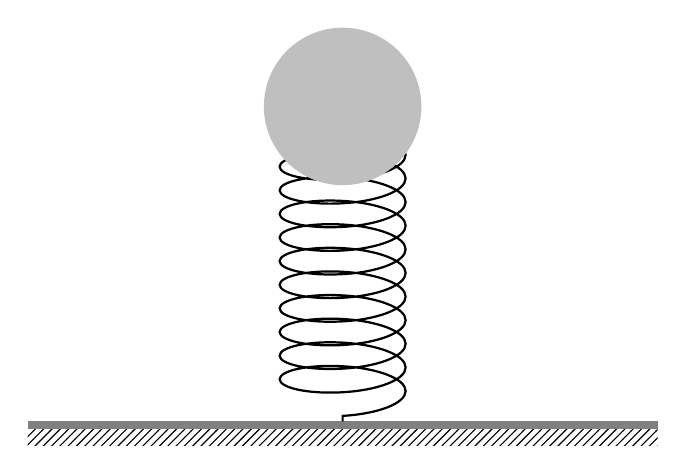
\begin{tikzpicture}[thick]
\newcommand{\ground}[2][]{
\begin{scope}[#1]
\usetikzlibrary{patterns,calc}
\def\groundlen{#2}
\fill[pattern = north east lines] (-#2,0) rectangle (#2,0.2);
\fill[color=black!50] (-#2,0.2) rectangle (#2,0.3);
\end{scope}}

\ground[yshift=-4.3cm]{4cm}
\draw[decoration={aspect=0.3, segment length=3mm, amplitude=8mm,coil},decorate] (0,0) -- (0,-4); 

\fill[gray!50] (0,0) circle (1);

%\fill (0,0) circle (0.1);
%\draw[thick,-latex] (0,0) -- (0,4) node[right] {$F$};
%\draw[thick,-latex] (0,0) -- (0,-3) node[right =1cm] {$G$};
\end{tikzpicture}

\end{document}